%
% The first command in your LaTeX source must be the \documentclass command.
\documentclass[sigconf]{acmart}
%\documentclass{acmart}

%
% defining the \BibTeX command - from Oren Patashnik's original BibTeX documentation.
\def\BibTeX{{\rm B\kern-.05em{\sc i\kern-.025em b}\kern-.08emT\kern-.1667em\lower.7ex\hbox{E}\kern-.125emX}}
    
% Rights management information. 
% This information is sent to you when you complete the rights form.
% These commands have SAMPLE values in them; it is your responsibility as an author to replace
% the commands and values with those provided to you when you complete the rights form.
%
% These commands are for a PROCEEDINGS abstract or paper.
\copyrightyear{2019}
\acmYear{2019}
\setcopyright{acmlicensed}
\acmConference[Final Project]{Machine Learning Final Project 2019}{May 05, 2019}{Notre Dame, IN}
 \acmBooktitle{Machine Learning Final Project 2019, May 05, 2019, Notre Dame, IN}
% \acmPrice{15.00}
% \acmDOI{10.1145/1122445.1122456}
% \acmISBN{978-1-4503-9999-9/18/06}

%
% These commands are for a JOURNAL article.
%\setcopyright{acmcopyright}
%\acmJournal{TOG}
%\acmYear{2018}\acmVolume{37}\acmNumber{4}\acmArticle{111}\acmMonth{8}
%\acmDOI{10.1145/1122445.1122456}

%
% Submission ID. 
% Use this when submitting an article to a sponsored event. You'll receive a unique submission ID from the organizers
% of the event, and this ID should be used as the parameter to this command.
%\acmSubmissionID{123-A56-BU3}

%
% The majority of ACM publications use numbered citations and references. If you are preparing content for an event
% sponsored by ACM SIGGRAPH, you must use the "author year" style of citations and references. Uncommenting
% the next command will enable that style.
%\citestyle{acmauthoryear}

%
% end of the preamble, start of the body of the document source.
\begin{document}

%\bibliography{/Users/ClayElmore/Desktop/mendeley/DMD_Literature.bib}

%
% The "title" command has an optional parameter, allowing the author to define a "short title" to be used in page headers.
\title{Stochastic Energy Market Price Forecasting with Recurrent Neural Networks}

%
% The "author" command and its associated commands are used to define the authors and their affiliations.
% Of note is the shared affiliation of the first two authors, and the "authornote" and "authornotemark" commands
% used to denote shared contribution to the research.

\author{Elmore, Clay}
%\authornote{Both authors contributed equally to this research.}
\email{celmore1@nd.edu}
\affiliation{%
  \institution{University of Notre Dame}
}

\author{Kopp, Grace}
\email{gkopp@nd.edu}
\affiliation{%
  \institution{University of Notre Dame}
}
%
% By default, the full list of authors will be used in the page headers. Often, this list is too long, and will overlap
% other information printed in the page headers. This command allows the author to define a more concise list
% of authors' names for this purpose.
\renewcommand{\shortauthors}{Elmore and Kopp, et al.}

% ============================================================================================================================= %
%														Abstract																       %
% ============================================================================================================================= %

\begin{abstract}
Energy market forecasting is a necessary for the functional operation of electricity markets across the globe. Because of large price swings in energy prices, sometimes as much as 4 times, there is a large economic opportunity for accurate forecasting to incur profit for energy users. However, these prices are notoriously hard to predict accurately because of the large stochastic nature inherent to the problem. In this paper we use Recurrent Neural Networks to forecast Day Ahead Market (DAM) prices in the California Independent System Operator (CAISO) in 2015. The study consists of forecasting 24 hour increments for a week in January for 100 different energy providers in the CAISO. Furthermore, a full year of prices is forecasted for a single Californian energy resource for all of 2015. We show that a full year's worth of forecasting in California has an average error of around 10\%. This is on par with current standards in traditional forecasting methods. It is also shown that Recurrent Neural Networks are more resistant to changes in market dynamics involving seasonal changes than traditional methods such as ARIMA or GARCH. 
\end{abstract}

%
% The code below is generated by the tool at http://dl.acm.org/ccs.cfm.
% Please copy and paste the code instead of the example below.
%
% \begin{CCSXML}
% <ccs2012>
%  <concept>
%   <concept_id>10010520.10010553.10010562</concept_id>
%   <concept_desc>Computer systems organization~Embedded systems</concept_desc>
%   <concept_significance>500</concept_significance>
%  </concept>
%  <concept>
%   <concept_id>10010520.10010575.10010755</concept_id>
%   <concept_desc>Computer systems organization~Redundancy</concept_desc>
%   <concept_significance>300</concept_significance>
%  </concept>
%  <concept>
%   <concept_id>10010520.10010553.10010554</concept_id>
%   <concept_desc>Computer systems organization~Robotics</concept_desc>
%   <concept_significance>100</concept_significance>
%  </concept>
%  <concept>
%   <concept_id>10003033.10003083.10003095</concept_id>
%   <concept_desc>Networks~Network reliability</concept_desc>
%   <concept_significance>100</concept_significance>
%  </concept>
% </ccs2012>
% \end{CCSXML}

% \ccsdesc[500]{Computer systems organization~Embedded systems}
% \ccsdesc[300]{Computer systems organization~Redundancy}
% \ccsdesc{Computer systems organization~Robotics}
% \ccsdesc[100]{Networks~Network reliability}

%
% Keywords. The author(s) should pick words that accurately describe the work being
% presented. Separate the keywords with commas.
\keywords{machine learning, stochastic forecasting, recurrent neural networks, energy markets}

%
% A "teaser" image appears between the author and affiliation information and the body 
% of the document, and typically spans the page. 
% \begin{teaserfigure}
%   \includegraphics[width=\textwidth]{sampleteaser}
%   \caption{Seattle Mariners at Spring Training, 2010.}
%   \Description{Enjoying the baseball game from the third-base seats. Ichiro Suzuki preparing to bat.}
%   \label{fig:teaser}
% \end{teaserfigure}

%
% This command processes the author and affiliation and title information and builds
% the first part of the formatted document.
\maketitle

% ============================================================================================================================= %
%														Intro  																       %
% ============================================================================================================================= %

\section{Introduction}
\label{sec:intro}

Energy markets are present all around the globe. Prices in these markets are extremely volatile due to a variety of different factors including but limited to market demand, erratic weather, natural resource availability, and so much more. Because of the large swings in these prices, participating in these energy markets presents an economic opportunity to both energy buyers and sellers alike. For an energy provider, knowing when the price of energy will be high is critical to knowing when to use valuable resources to produce energy. For an energy user, knowing when to buy energy on the market at a low price can be the difference between an industrial user being profitable or going under. With these considerations in mind, it is clear that energy price forecasting is a worthy venture for academics to study because of its direct applicability to the commercial world.\\

In this paper, we will explore a specific energy market: the California Independent System Operator (CAISO). The CAISO is an enormous, complex energy market system in which energy buyers and sellers schedule a multitude of energy related transactions. The CAISO had some 40 billion dollars in sales, and more than 260,000 gigawatts sold in 2015\cite{CAenergy2}. This complex system makes for a data-rich problem worthy for study by academics and industry professionals alike. A particularly interesting problem in the CAISO is the forecasting of Day-Ahead Market (DAM) prices which are notoriously stochastic. DAM prices are used to forecast energy prices a day in advance which energy buyers and sellers then use to schedule when they will buy and sell energy on the CAISO market. It has been shown that accurate forecasting is absolutely critical to profiting off DAM market prices\cite{Dowling2017}.\\

Although prices in the CAISO DAM are quite volatile, they have very clear periodic tendencies. Figure \ref{fig:ex_prices} shows an example week of energy prices for an energy resource in the CAISO DAM for the first week of 2015. Note how the price is clearly periodic, but also has stochastic tendencies as well. Furthermore, Figure \ref{fig:ex_prices} shows the economic opportunity available to sell at high prices and buy at low prices. Some price swings are almost double the price. An accurate forecast would allow for large amounts of profit to be extracted from these systems.\\

\begin{figure}[h]
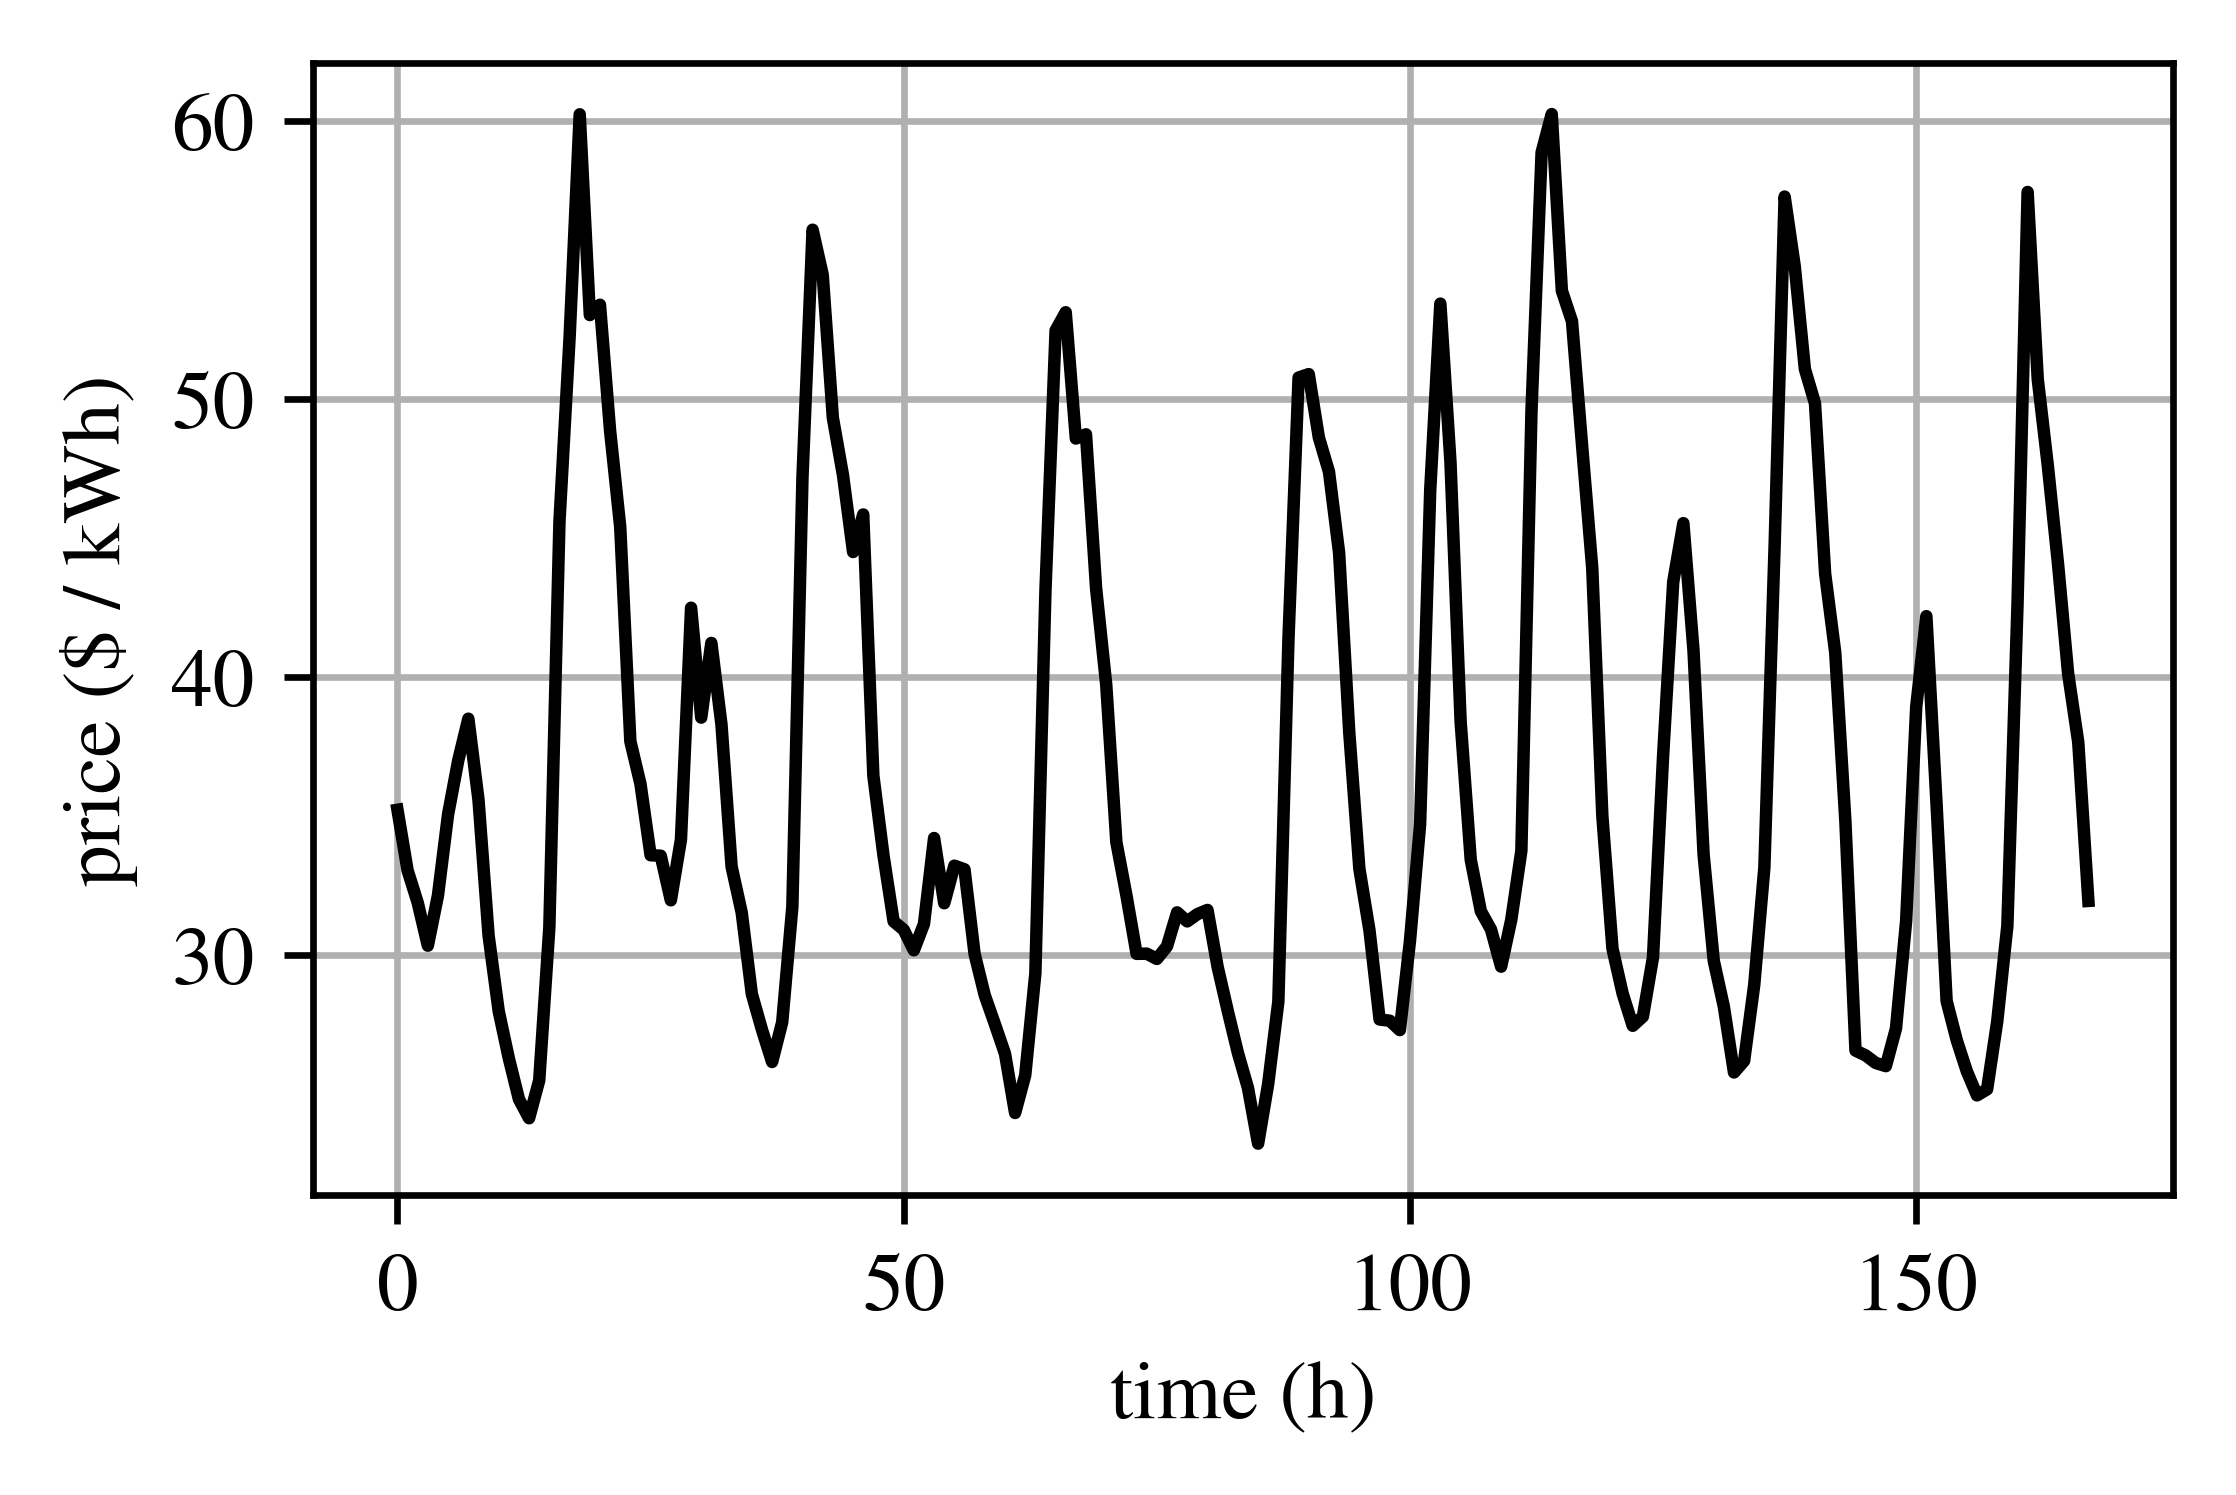
\includegraphics[width=0.45\textwidth]{fig_1.png}
\caption{An example of time series behavior observed in the CAISO from January 1st, 2015 to January 7th, 2015.}
\label{fig:ex_prices}
\end{figure}

Recent advances in Recurrent Neural Networks (RNN) in the past 5 to 10 years have motivated this project to investigate their potential ability to predict CAISO DAM prices. The remainder of the paper will be organized in the following manner.

\begin{itemize}
	\item Section \ref{sec:work}: A short introduction to some related work based on traditional methods of time series forecasting energy prices.
	\item Section \ref{sec:approach}: A problem statement along with the design of the RNN, an explanation of the dataset, and software implementation details.
	\item Section \ref{sec:results}: Results of the forecasting performance of our RNN forecaster is presented along with a discussion of how RNN forecasting compares to existing methods and other insights from this project.
	\item Section \ref{sec:conclusions}: Major findings from the paper are summarized.
\end{itemize}

The main contribution of this paper is to show that RNNs are a viable way to forecast energy market prices. Furthermore, the RNN's used in this paper are shown to have lower error rates than standard forecasting methods such as GARCH and ARIMA. 

\section{Related work}
\label{sec:work}

Many standard time series forecasting methods have been used to predict DAM prices in the CAISO and other energy markets across the globe. For example, standard autoregressive integrated moving average (ARIMA) forecasting methods have been used to differing degrees of success in the CAISO market and the Spanish DAM. Conejo et al. have used ARIMA models to predict prices in the Spanish market with a 10\% error for the 2002 market \cite{Conejo2005a}. Furthermore, ARIMA has been shown to generate forecasts in the 2000 CAISO DAM with an error of around 13\% \cite{Garcia2005}. Another standard method for time series forecasting that has been used in the  Generalized autoregressive conditional heteroskedasticity (GARCH) method. Similar to ARIMA models, an error rate of around 10\% for the Spanish DAM has been reported when using GARCH \cite{Garcia2005}. More advanced hybrid methods have also been used for DAM forecasting. These methods include the usage of wavelet decompositions in order remove noise from data as well as the incorporation of ARIMA models in conjunction with GARCH methods \cite{Conejo2005,Tan2010,Amjady2008,Wang2012}. These various hybrid methods have error rates reported that range from as low as 1\% to as high as 25\%. 

% ============================================================================================================================= %
%														Approach																       %
% ============================================================================================================================= %

\section{Method / Approach}
\label{sec:approach}

\subsection{Problem Statement}
We set out to use a recurrent neural network to forecast Day Ahead Market (DAM) prices of the California Independent System Operator (CAISO)  in 2015. Specifically, we wanted to forecast 7 24 hour increments for a week in January for 100 different energy providers in the CAISO. 

We also set out to get in depth information on one energy provider so we forecasted a full year (2015) of prices for one energy provider.

\subsection{Neural Network Methodology}
We used a recurrent neural network (RNN) for our time series prediction. We chose to use this architecture because RNNs are made to deal with sequential information. In other neural network architectures, it is assumed that all inputs are independent which would not be useful for a time series prediction where the order of the inputs is extremely important to accurately predict outputs. RNNs accomplish this by keeping a “memory” of inputs they have seen at previous time steps to make decisions about future time steps \cite{Dasgupta2018}.  

\begin{figure}[h]
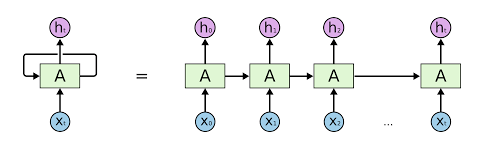
\includegraphics[width=0.45\textwidth]{rnn.png}
\caption{An unrolled recurrent neural network cell \cite{Dasgupta2018}.}
\label{fig:rnn}
\end{figure}

Figure \ref{fig:rnn} depicts an unrolled RNN. For a sequence with t time steps, we will unroll our network into t corresponding layers. The blue nodes labelled x1,  x2, etc. are our inputs at time step one, two, and so on. In the case of this paper, these would be energy prices at hour 1, hour 2, etc. The green nodes labelled A are our hidden states at each time step. This is how the network is able to have a memory. It is calculated with the previous hidden step and the current input. Because it takes this previous hidden step into account, it captures information about time steps that have already been processed. Finally, the purple nodes labelled with h’s are the outputs at each time step that are calculated from the memory in their associated hidden node. For us, these outputs are the energy prices we are predicting for future time steps. 

Unfortunately, basic RNNs are not perfect for this task because of the vanishing gradient problem. RNNs are trained with back propagation and gradient descent learning methods. When dealing with a huge number of time steps, as is the case in our dataset, calculated gradients can become so small that the neural network is unable to continue to train. 

Our solution to this problem was using a Long-short Term Memory network (LSTM). These are a type of neural network that have input gates, output gates, and forget gates that give the network the ability to keep some information while forgetting other information. This cuts down the amount of data used and solves the vanishing gradient problem \cite{Dasgupta2018}. 

We wanted to be able to forecast a days worth of energy prices in advance or 24 output time steps. To accomplish this, we created a Multi-Step LSTM where our output was a vector of 24 prices corresponding to the 24 time steps in the future we predicted \cite{Brownlee2018}. Our training data was the 168 time steps (one weeks worth) of data that came directly before the 24 hour testing period.

In order to get an accurate view of our network and match other current evaluation models for energy price forecasting, for each of the fifty nodes we analyzed, we performed a rolling horizon analysis to predict seven days worth of data. In other words, first we used $t_{0}$ through $t_{167}$ to predict $t_{168}$ through $t_{191}$ , then we used $t_{24}$ through $t_{191}$ to predict $t_{192}$ through $t_{216}$ , and so on five more times until we had seven days of predictions or 168 hours.

To calculate error, we performed a standard average percent error calculation on our predicted prices vs the actual price. We chose percent error in order to be able to easily compare our results to other energy forecasting results on the same data from different prediction methods.

\begin{equation}
error = \frac{1}{7}\sum_{i=0}^{6}\frac{1}{24}\sum_{j=0}^{23}\frac{|p_{i,j}-a_{i,j}|}{a_{i,j}}
\end{equation}

In the above equation $p_{i,j}$ is the predicted energy price on day i, hour j and $a_{i,j}$ is the actual energy price on day i, hour j.

As a supplemental inquiry, we also investigated forecasting a full year of energy prices for one energy provider. This was done almost identically, except for this study we used 336 input time steps as training to predict 24 hour time step outputs. We performed this calculation 356 times to see how our RNN performs on more long term data. Error was calculated using the same method above except for 365 days instead of 7:

\begin{equation}
error = \frac{1}{365}\sum_{i=0}^{364}\frac{1}{24}\sum_{j=0}^{23}\frac{|p_{i,j}-a_{i,j}|}{a_{i,j}}
\end{equation}


\subsection{Software Implementation}
This study was implemented using Keras with a TensorFlow backend. Specifically, we used the sequential library in the Keras packaged to define and train our LSTM model. We chose to use Keras because it is allowed us to access the deep learning resources of TensorFlow in an easy to use API. Because we were dealing with a huge amount of data, our study had a very high computation time. To make this more manageable, we submitted our code as jobs to the University of Notre Dame Center for Research Computing GPUs. This allowed faster and more convenient processing than if we were to run our model locally. Our entire code suite  is available at https://github.com/celmore25/neural\_net\_predictions. This includes our class implementation of the model, our data, our evaluation tool, and every other piece of code we wrote in pursuit of completing this study. This research was supported in part by the Notre Dame Center for Research Computing through the use of available GPU systems. 

\section{Data}
The dataset for this project was kindly provided by the Dowling Lab for Uncertainty Quantification and Mathematical Optimization at the University of Notre Dame in the Department of Chemical and Biomolecular Engineering. The dataset is comprised of over 6500 energy vendors, called nodes, participating in the CAISO. There is a full year's worth of data for each node in 2015, and price measurements are recorded at 1 hour intervals. Latitude and longitude coordinates are known for around 2000 of these nodes for visualization purposes. Because of the limited timeline of this project, only 100 of these nodes will be used, and only a single week of data in January 2015 will be used for testing purposes.  This is a reasonable thing to do as many papers report error values for single weeks in January \cite{Conejo2005a,Garcia2005,Tan2010}. However, a single node will be used to predict prices 24 hours into the future for a full year in order to give a more accurate representation of error quantification across a larger time span. Furthermore, these papers only report results for single nodes in the DAM. Because our results include 100 nodes, it can be concluded that the results obtained for this dataset are statistically significant. 


% ============================================================================================================================= %
%														Results																       %
% ============================================================================================================================= %
\section{Evaluation}
\label{sec:results}

Now that we have shown how we are going to forecast market prices with a RNN, we will now enter the results section where we analyze the effectiveness of RNNs. 

\subsection{Example Forecasts}

It is important to notice that variations in market prices can significantly alter the ability of RNNs to accurately predict DAM prices. Figure \ref{fig:ex_forecast} was constructed by training a RNN with 336 hours of training data, or two weeks. This 336 hour training set was then split into 265 training instances. These instances consisted of one 24 hour input, and the corresponding 24 hour output that would be the next day's market data. Two different forecasts are shown in Figure \ref{fig:ex_forecast} to illustrate how different inputs to the RNN can drastically alter its ability to forecast market prices. In the first plot (top), there is well behaving periodic wave input to the RNN. The output is a forecast that is extremely successful with a small error of only 4.4\%. However, the second plot (bottom) shows that when there is an input that does not behave as well. Without the direct sinusoidal behavior, the RNN struggles to accurately predict the price at an error of 27\%. Based on this analysis, it will be important to look at aggregated results from more than two forecasts in order to show how well an RNN actually performs in forecasting the CAISO DAM.

\begin{figure}[h]
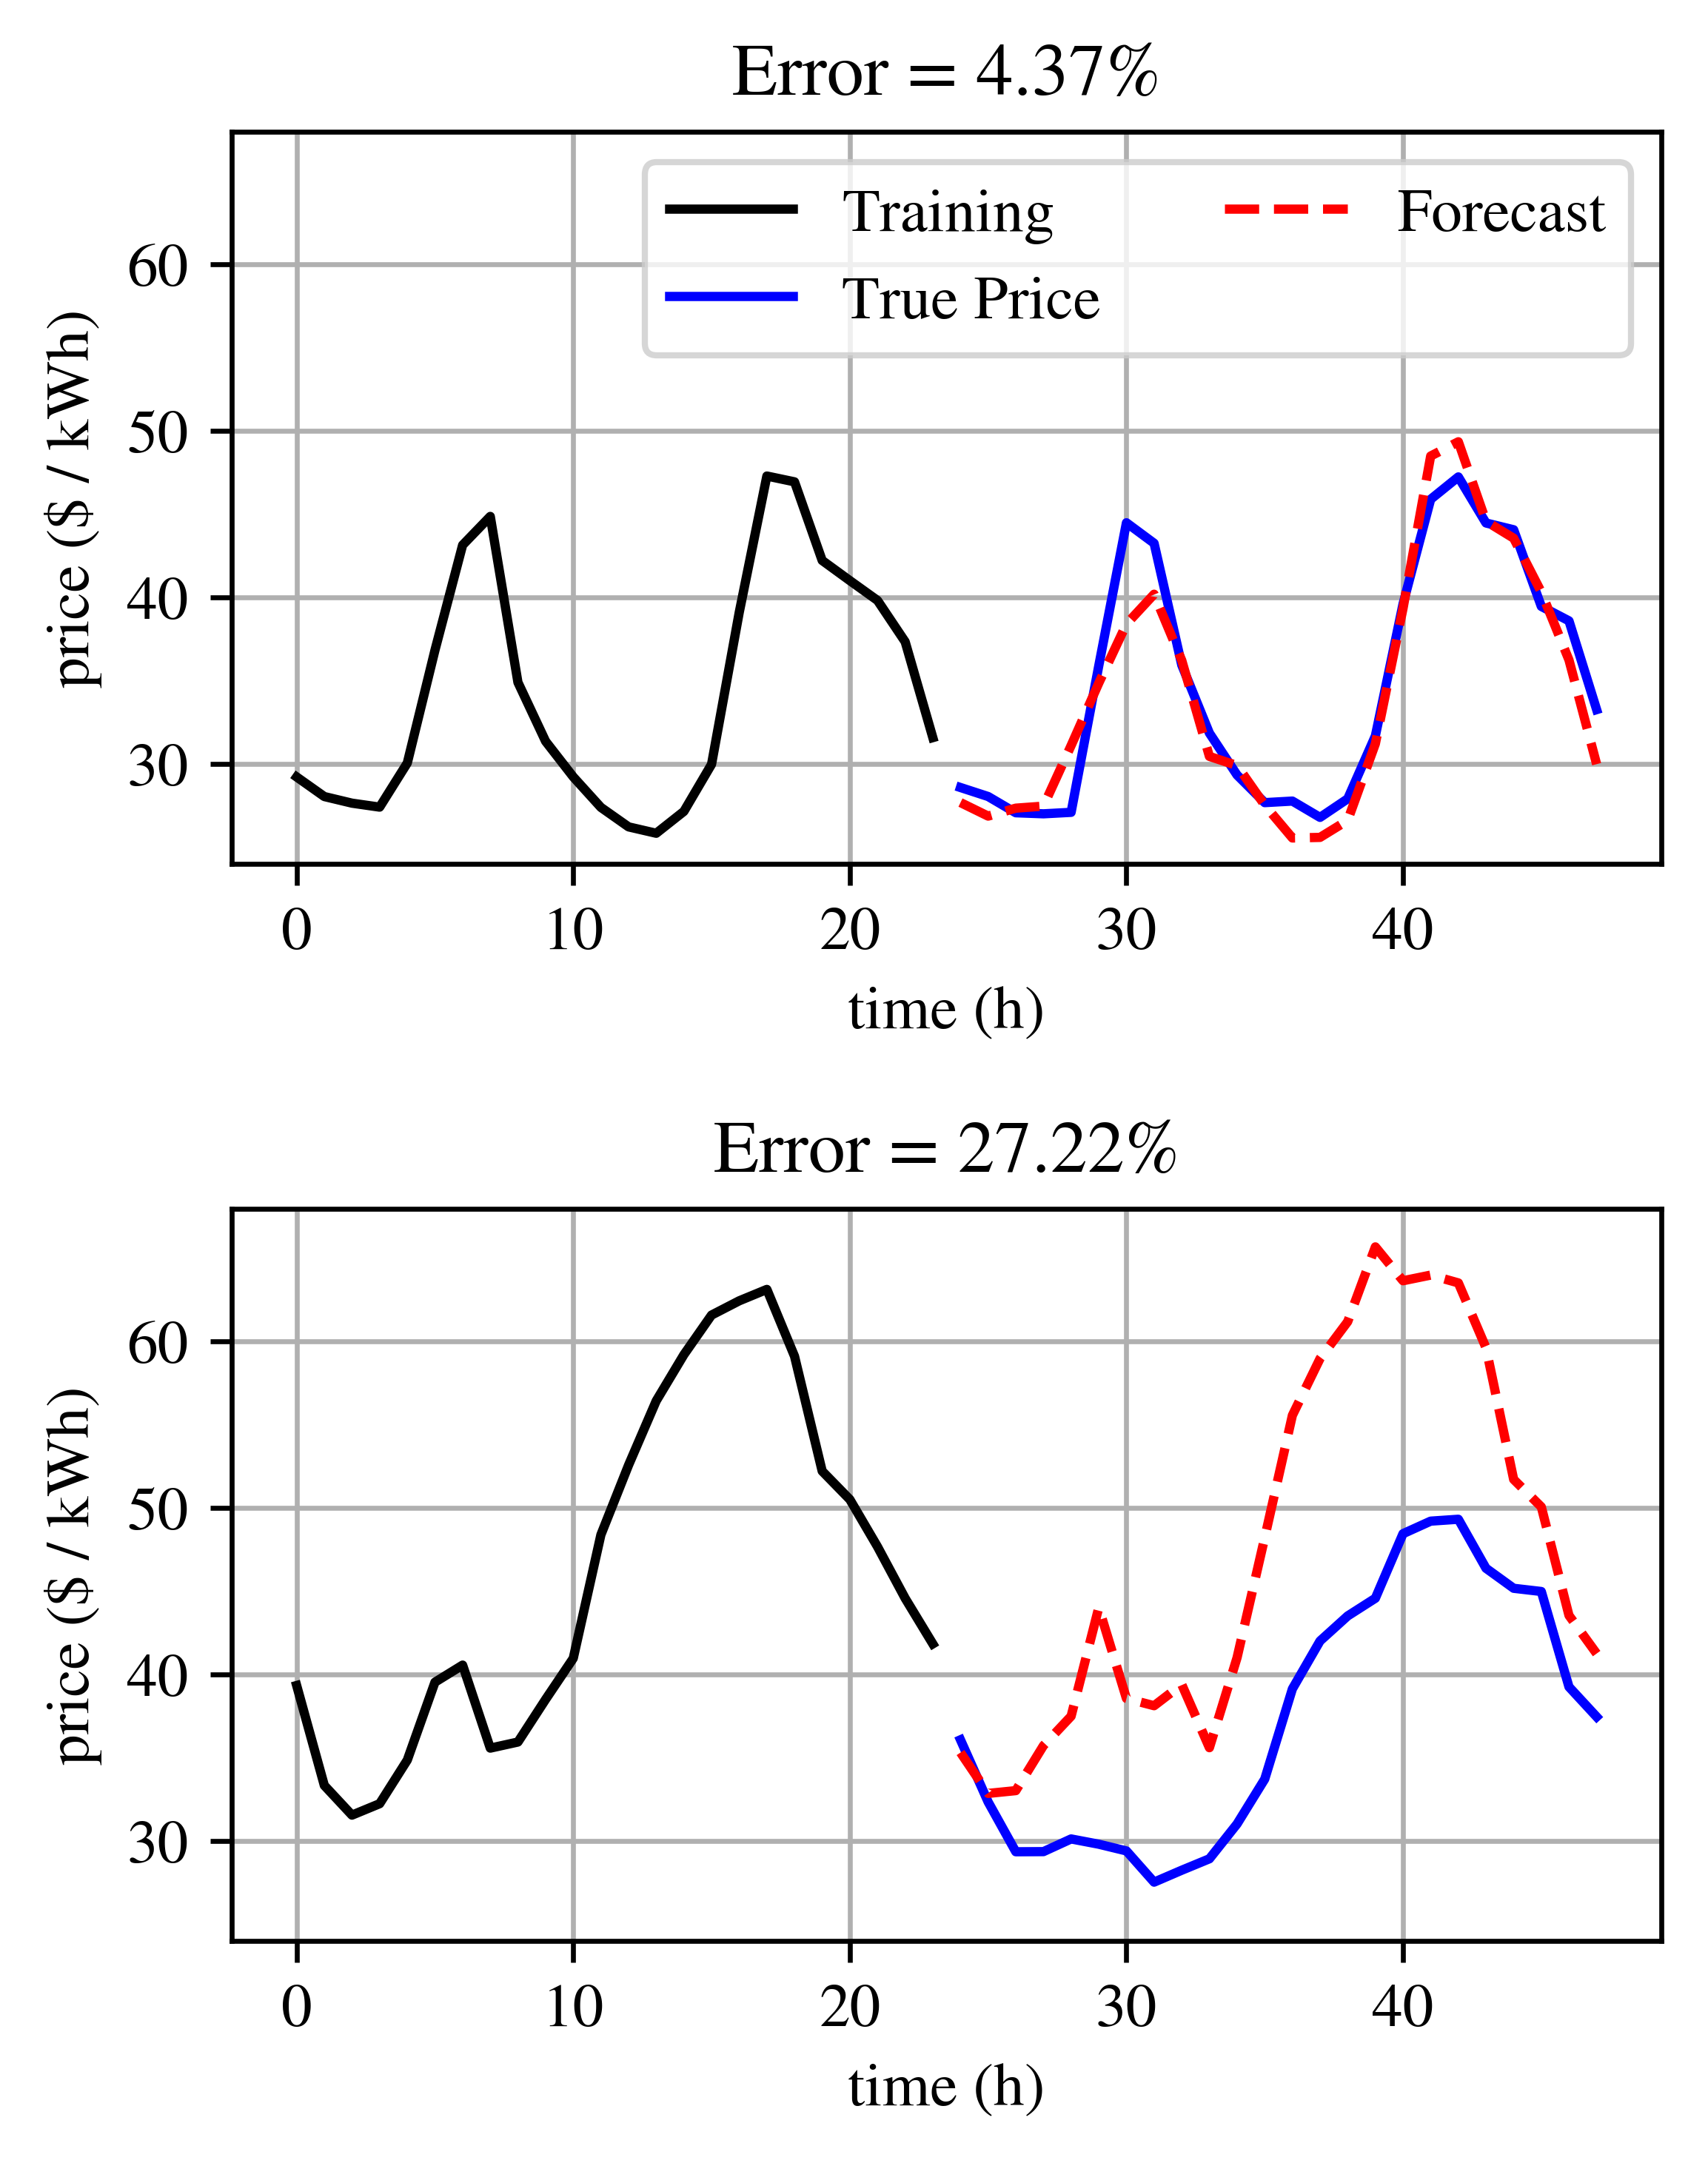
\includegraphics[width=0.45\textwidth]{fig_3.png}
\caption{Example price forecasting using our RNN.}
\label{fig:ex_forecast}
\end{figure}

\subsection{Multiple Node, Single Week Forecasts}

With Figure \ref{fig:ex_forecast} motivating the exploration into aggregated results from the dataset, Figure \ref{fig:hist_small} shows a histogram of the forecasting results of 100 nodes in the CAISO for a single week in January. This histogram was created by training 100 separate RNNs on 168 hours of training data for each individual node. These RNNs then predict 24 hours into the future and an error measurement is taken based on the true data. The horizon is then rolled into the future for 7 days in a row, and the error measurements for a week are averaged to give the results in Figure \ref{fig:hist_small}. Figure \ref{fig:hist_large} is generated by doing the exact same analysis except this time the RNN is training with two weeks (336 time series points). The histograms shows the error is reasonably dependent on the node being forecasted. This is most likely due to different spatial dependencies in price points across California. These influences can include weather, natural resource availability, etc. Because of these natural variations, it is expected that each node has a very different performance. Furthermore, the histograms show how the RNN generally performs better when supplied with a larger data input.

\begin{figure}[h]
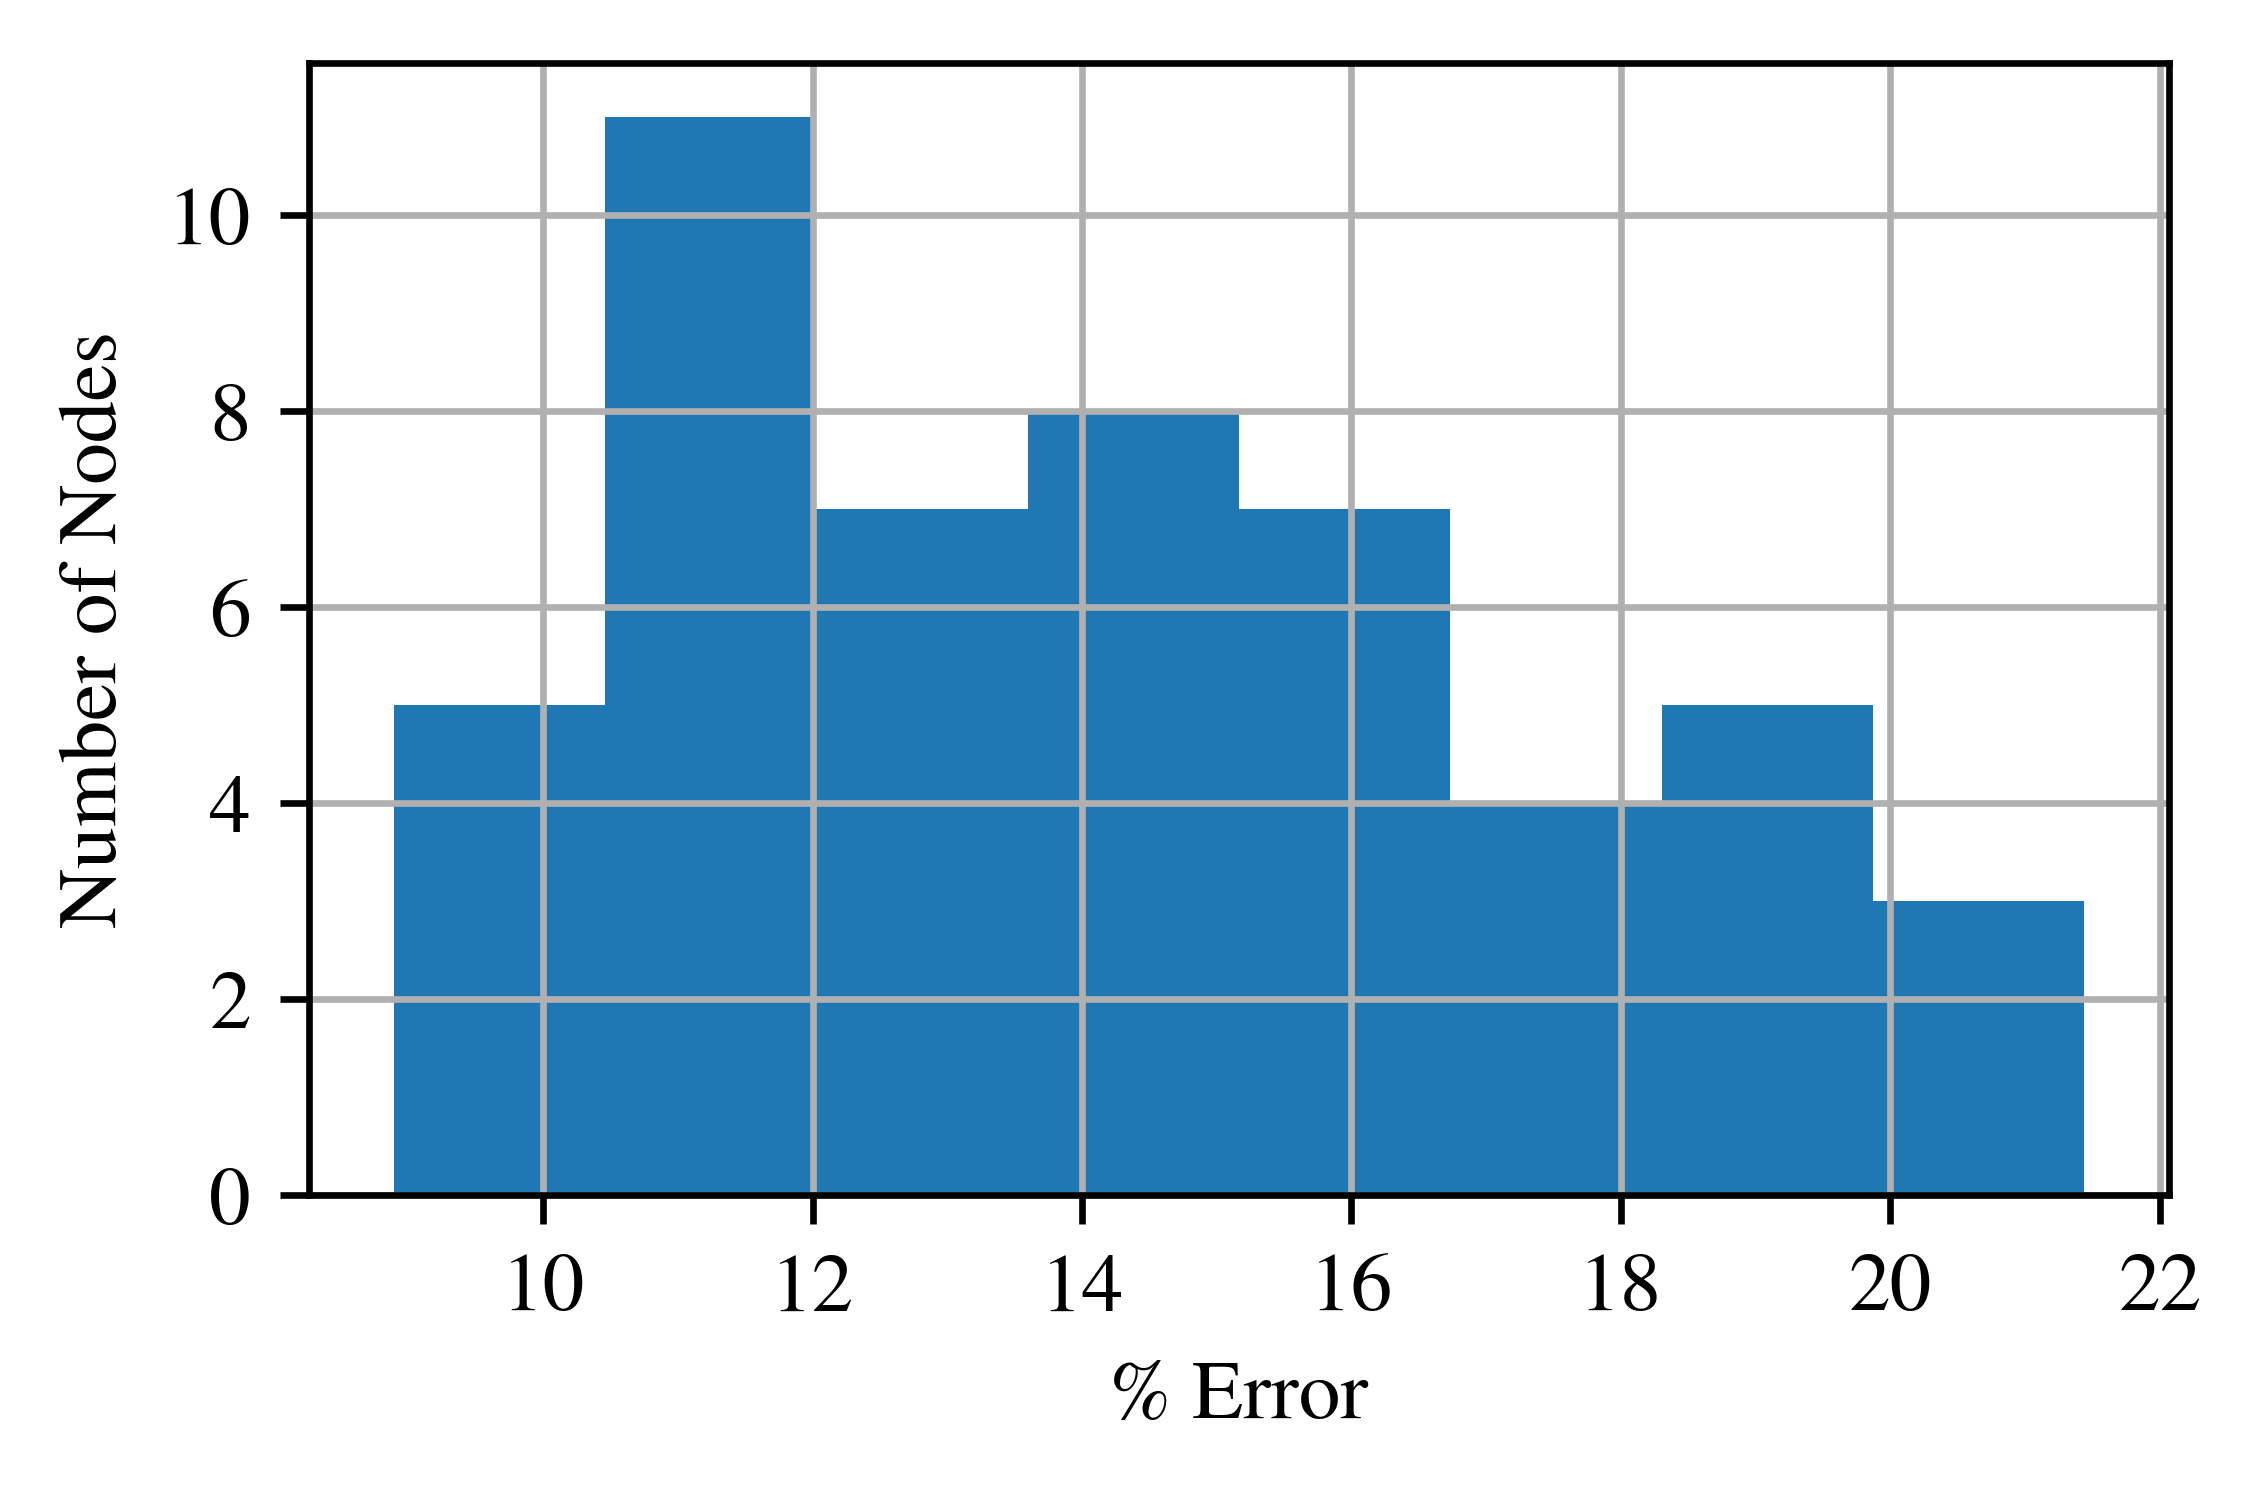
\includegraphics[width=0.45\textwidth]{fig_5.png}
\caption{Histogram of all nodes' results at forecasting a week of data in January 2015 using one week of training data.}
\label{fig:hist_small}
\end{figure}

\begin{figure}[h]
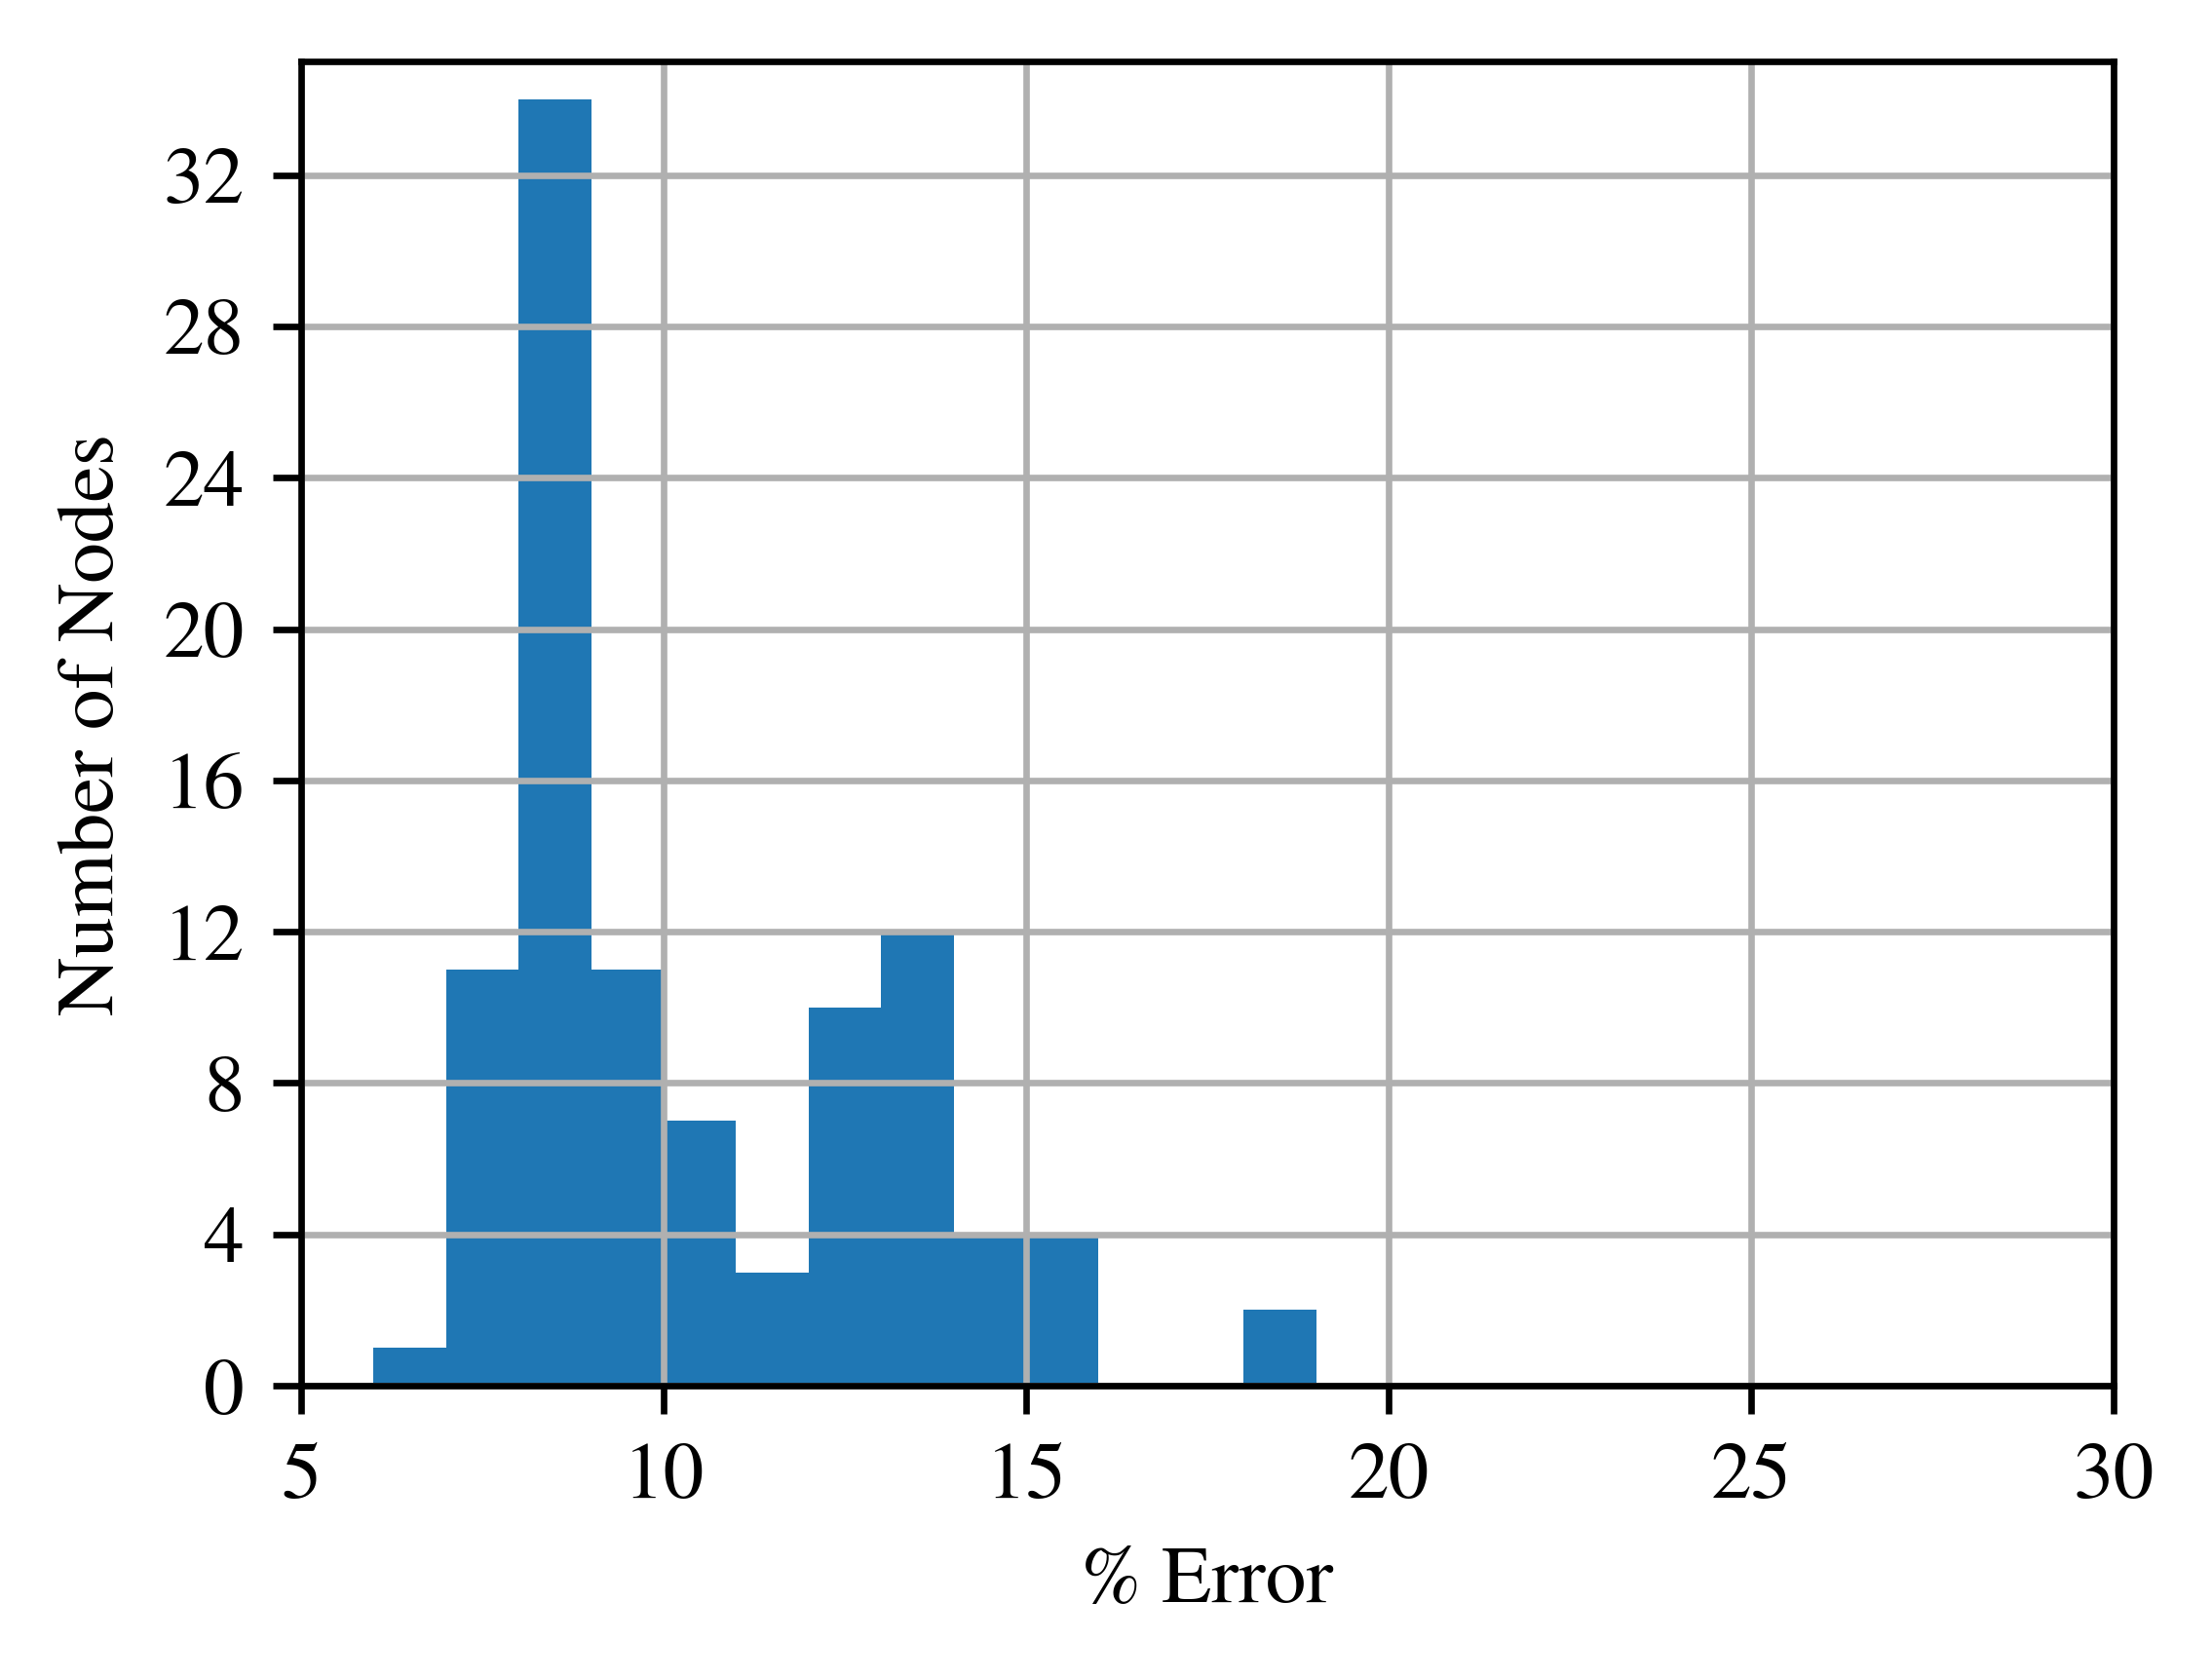
\includegraphics[width=0.45\textwidth]{fig_5_1.png}
\caption{Histogram of all nodes' results at forecasting a week of data in January 2015 using two weeks of training data.}
\label{fig:hist_large}
\end{figure}

Table \ref{tab:all_nodes} provides some aggregated statistics for the single week performance of a RNN across 100 different nodes. An error rate of 14\% is similar to literature values reported for certain single weeks in the CAISO from various literature findings that were mentioned in the introduction. However, this is not beating current standards of forecasting with traditional ARIMA models. However, when two weeks of training data is used to train the RNN, the forecasting error drops to 10.6\% which is about on par with standard time series methods. In order to look further into how effective RNN forecasting is, a single node is investigated more in depth in the next section.

\begin{table}[h]
\begin{tabular}{lll}
\hline
\hline
Training Data Used & 1 week & 2 weeks \\
\hline
Median             & 12.65  & 9.18     \\
Mean               &  13.70 & 10.64     \\
Standard Deviation & 3.44   & 3.28    \\
\hline
\hline
\end{tabular}
\caption{Aggregated statistical performance for a single week in January when 1 week of training data was used vs. 2 weeks of training data.}
\label{tab:all_nodes}
\end{table}

\subsection{Single Node, Full Year Forecasts}

As previously mentioned, it is desired to look at a single node's performance in RNN forecasting for the whole year in 2015. Figure \ref{fig:hist_single} was constructed by using 336 hours of rolling training data for a single node in the CAISO. A different RNN was trained for each rolling horizon, and the subsequent 24 hour forecast was recorded. The histogram shows the error rate as a function of the number of times it occurred. A first observation on Figure \ref{fig:hist_single} is that the dataset is very skewed to the right. From a market perspective, this means the RNN forecasts were generally quite accurate, but there were some large errors that did occur. It should also be noted that a large outlier at around 200\% is not shown in this graph. However, the overall accuracy of the test was quite good. The median error for the full year was only 9\% which is lower than previously reported for forecasting the CAISO via ARIMA and GARCH modeling \cite{Conejo2005a,Garcia2005}. 

\begin{figure}[h]
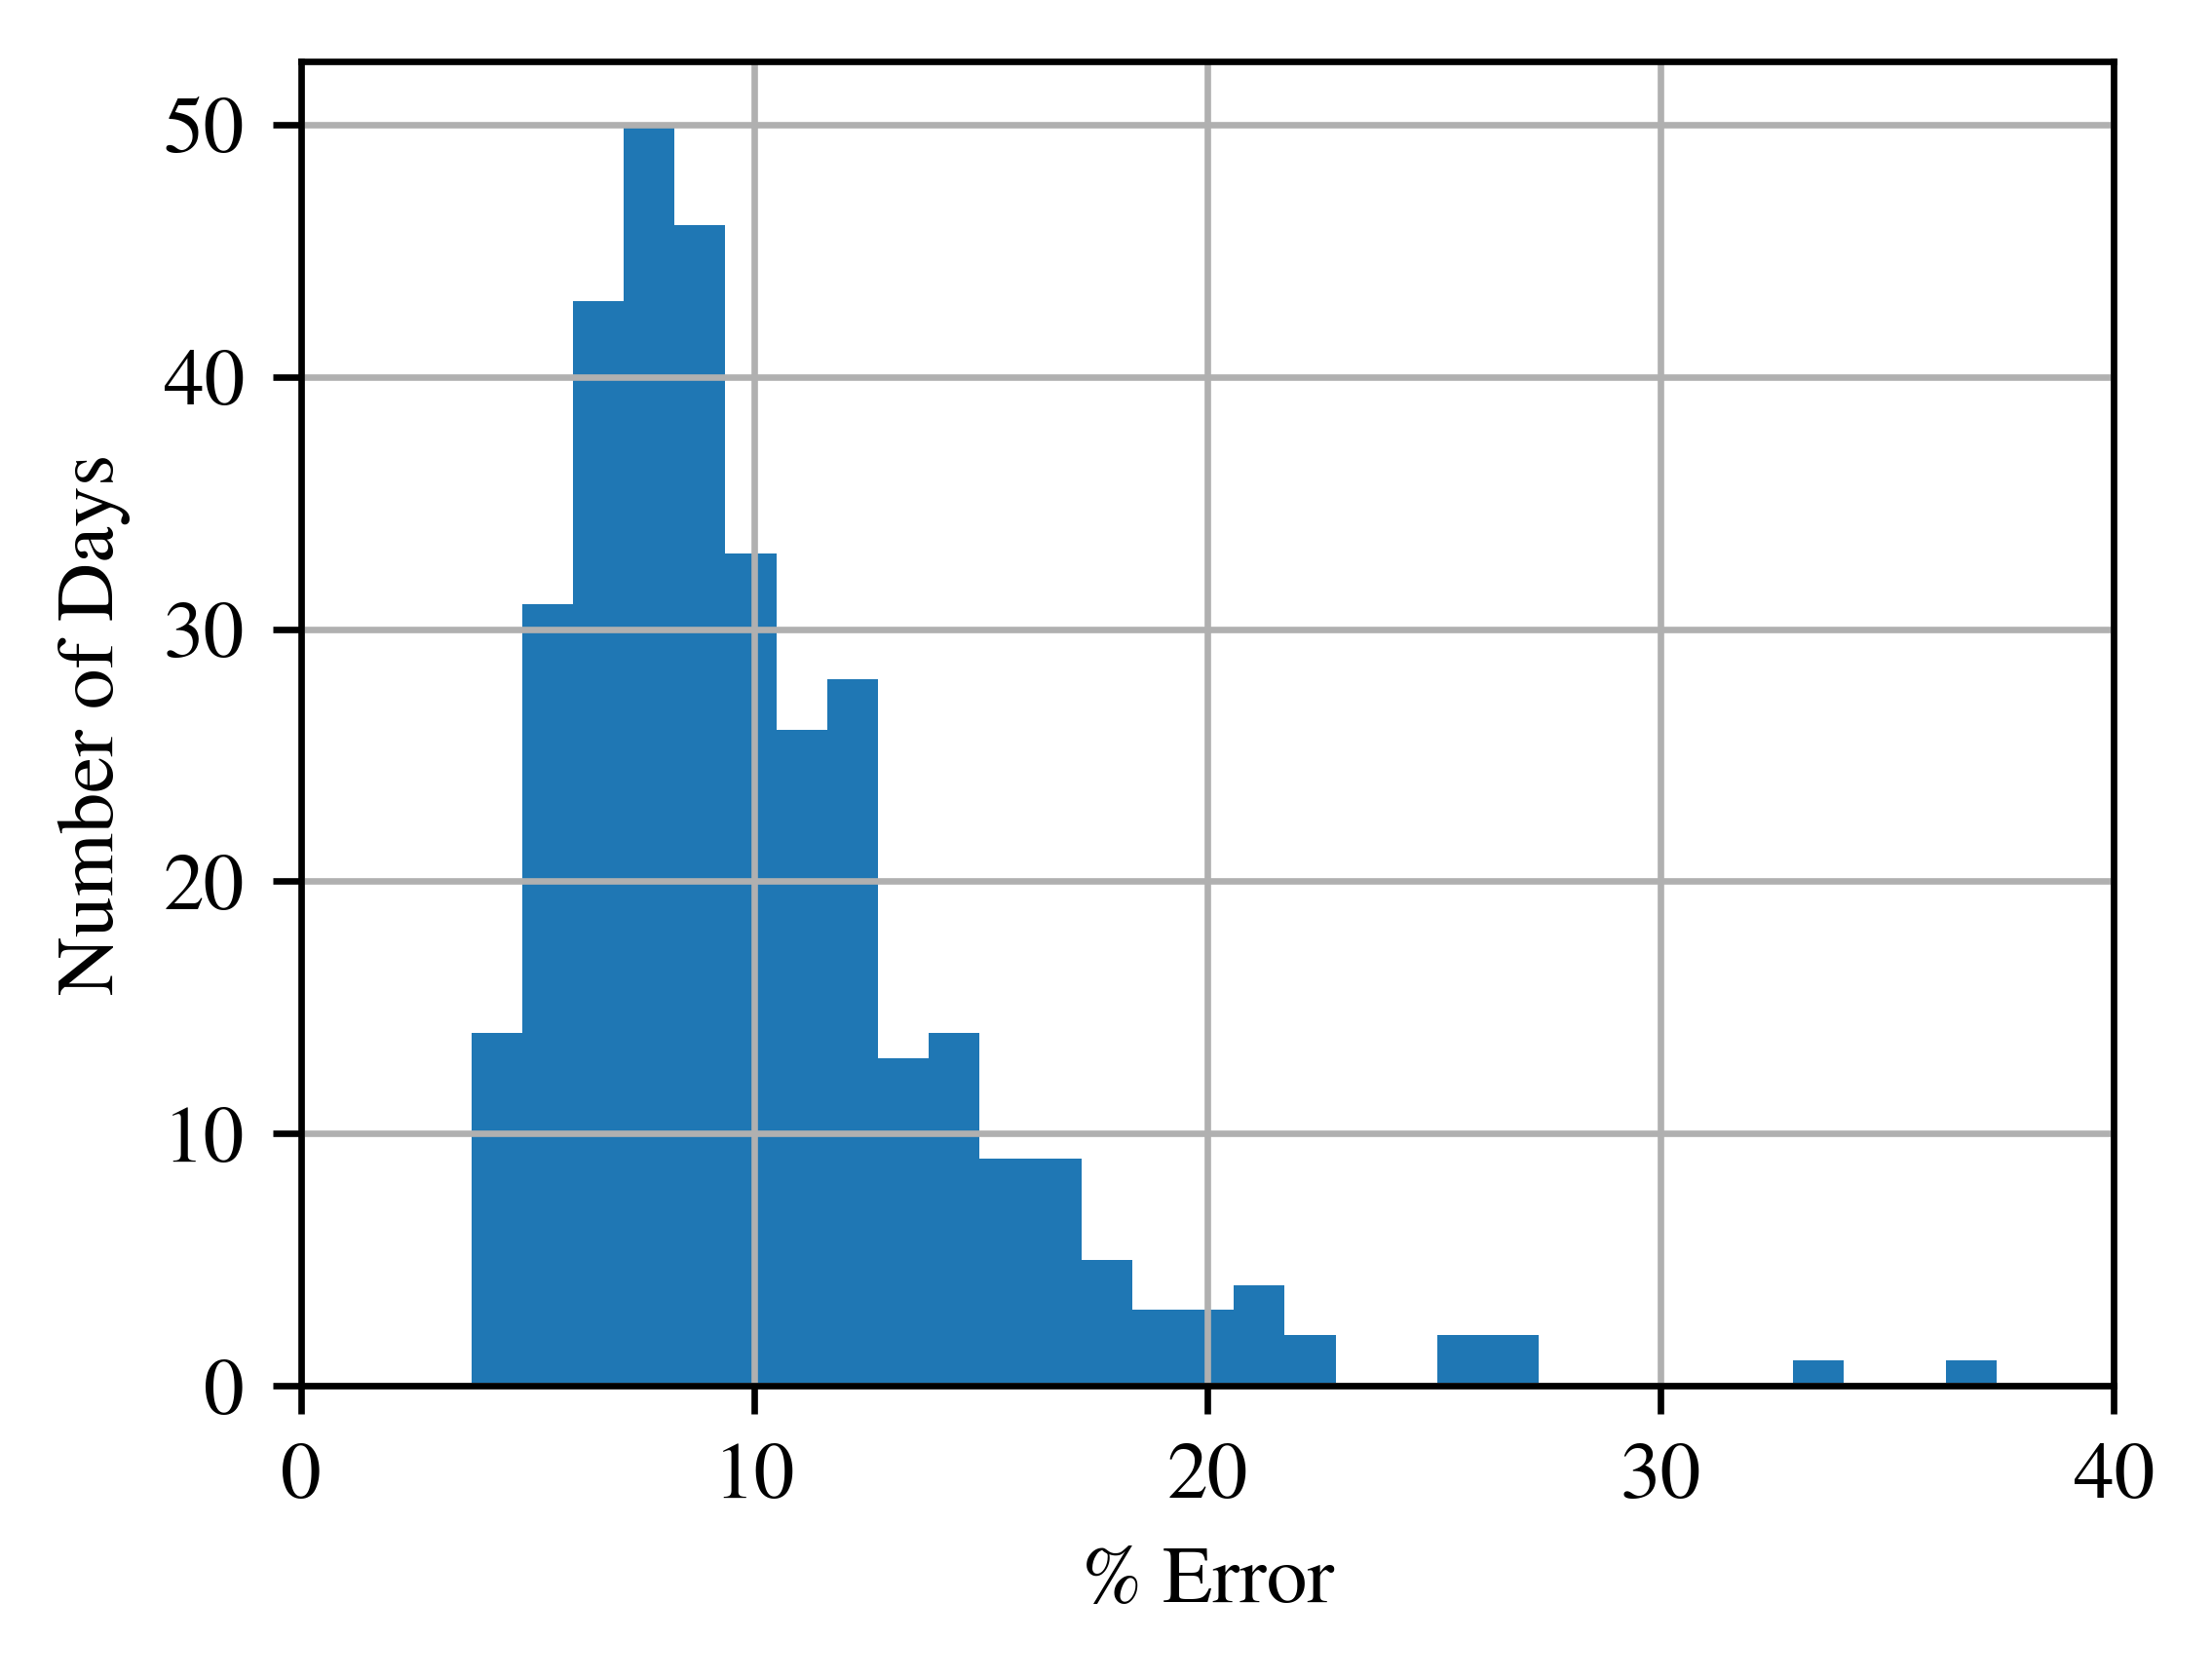
\includegraphics[width=0.45\textwidth]{fig_7.png}
\caption{Histogram of a single node run through the whole year.}
\label{fig:hist_single}
\end{figure}

An important thing to look at in the CAISO market is the tendency for the market to change between the seasons. It is well documented that price ranges are quite different in the four quarters of the year. To connect this observation with how well our RNN performs, Figure \ref{fig:time_single} plots the error of each day in forecasting across the whole year of 2015. An observation made from this graph is that the error does not seem to be very dependent on the seasonality of the data. There are some abrupt error jumps, but those are most likely due to natural market disturbances, not seasonal variations. 

\begin{figure}[h]
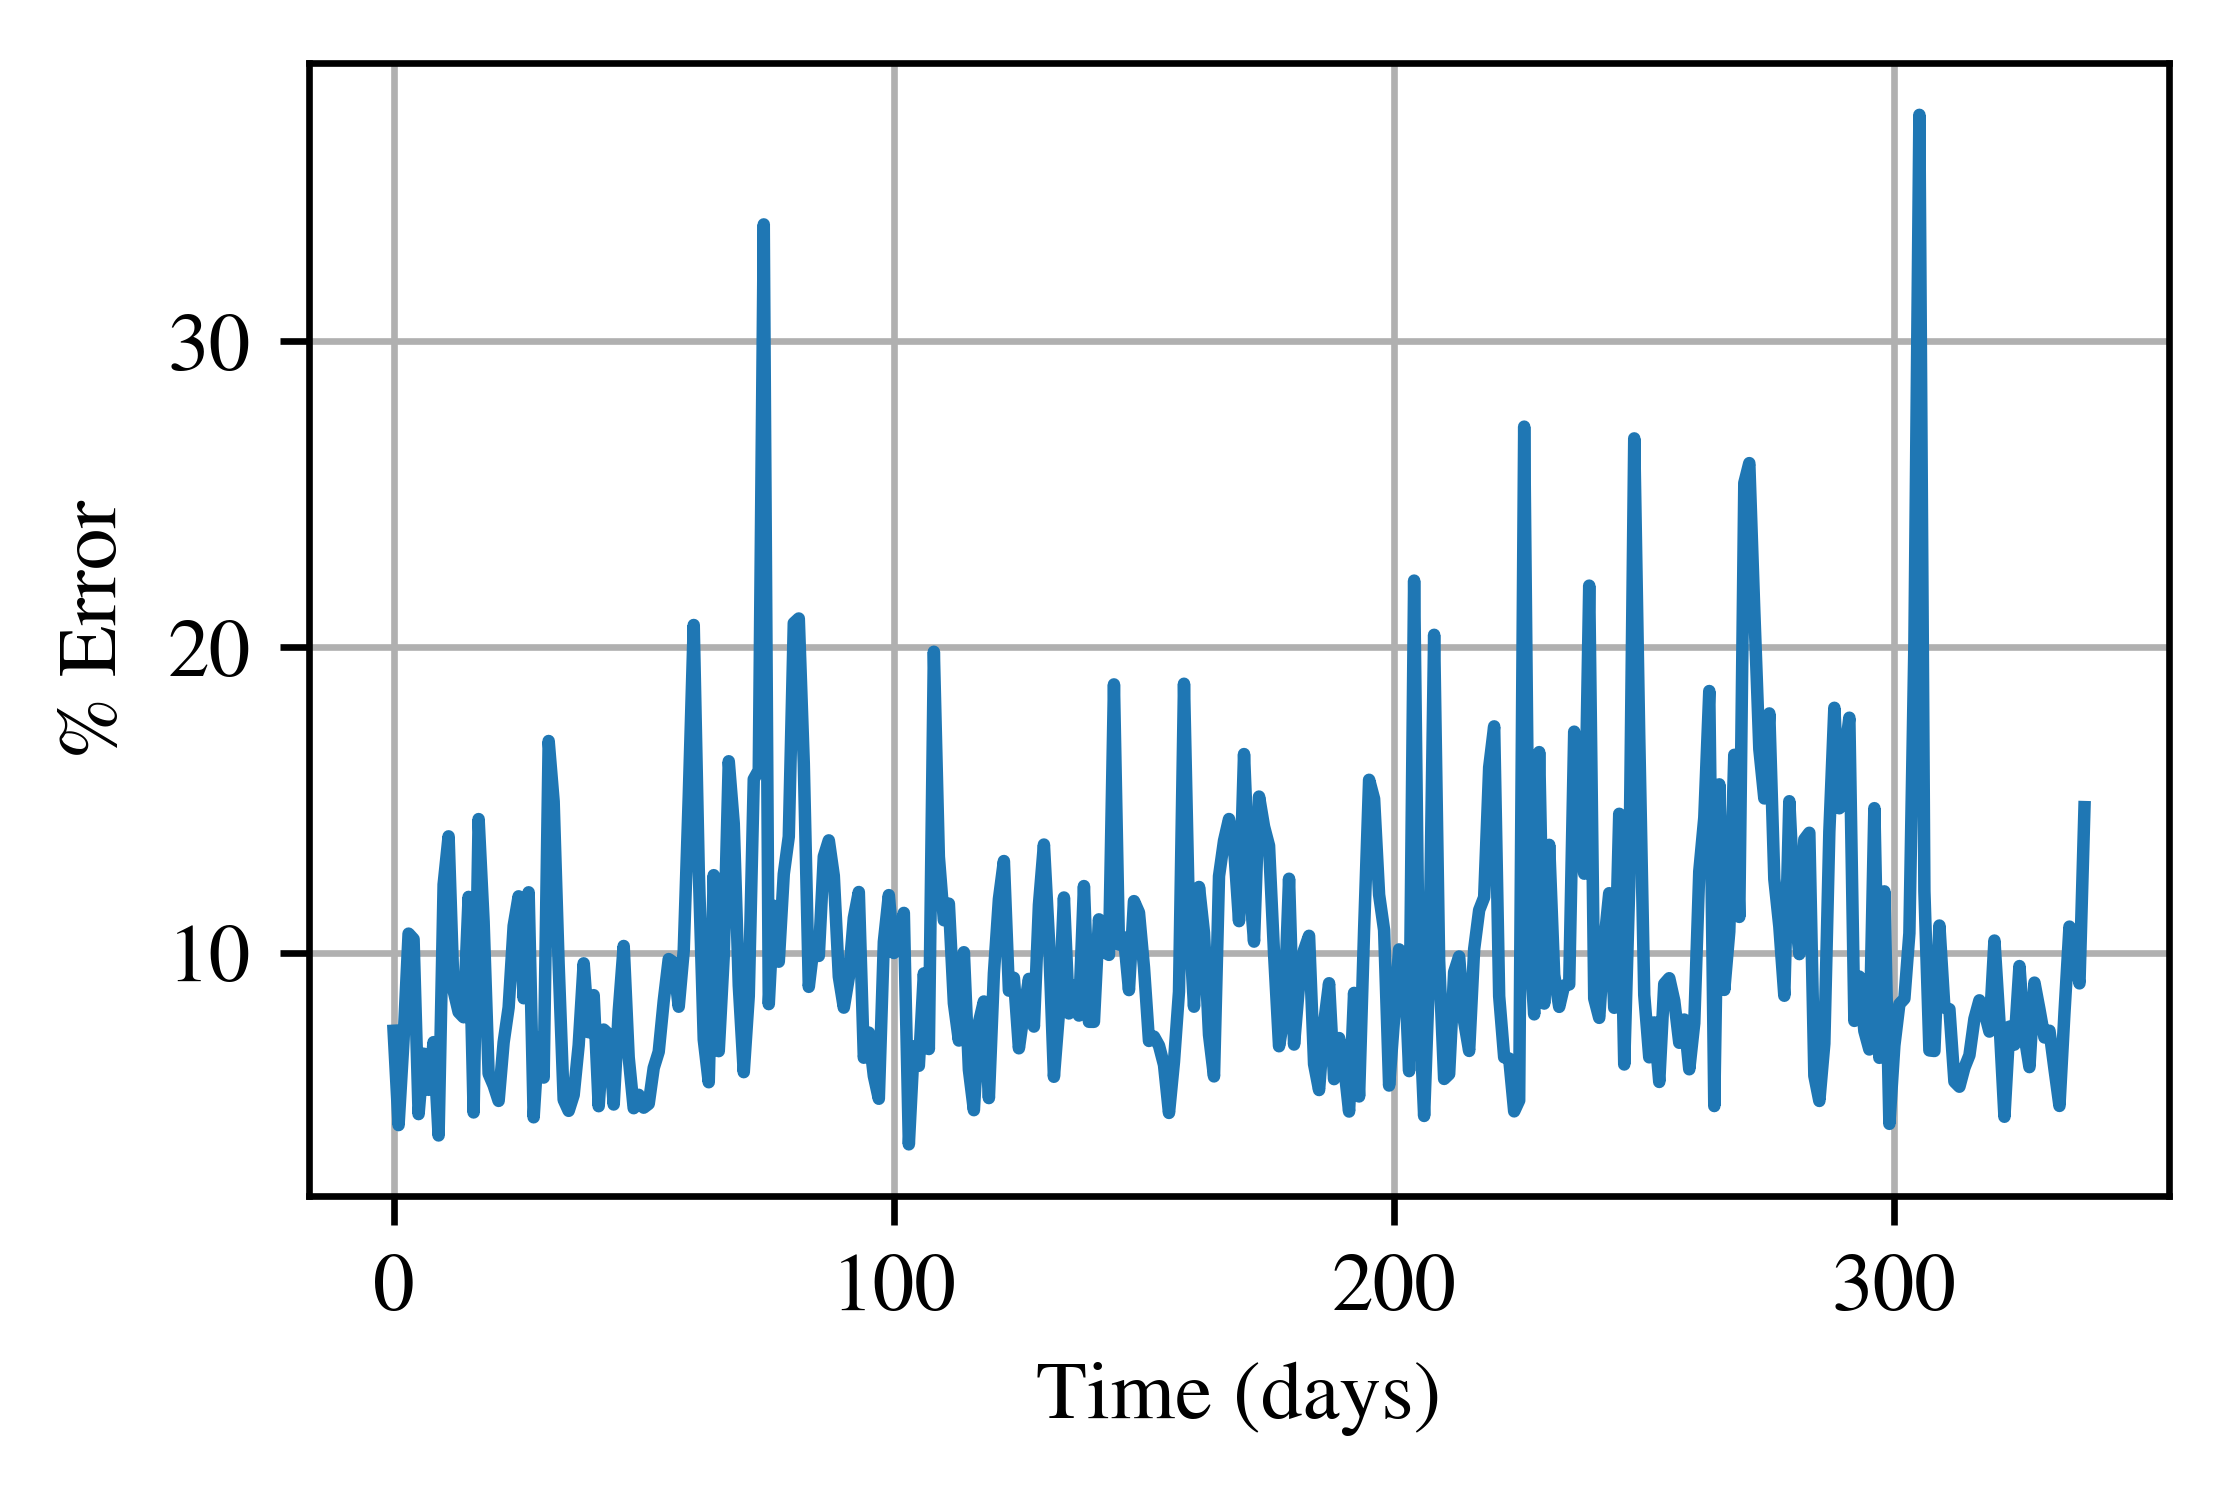
\includegraphics[width=0.45\textwidth]{fig_8.png}
\caption{Time series plot of a single node run through the whole year.}
\label{fig:time_single}
\end{figure}

Table \ref{tab:single} gives some aggregated results on the results shown in Figures \ref{fig:time_single} and \ref{fig:hist_single}. The qualitative observation that seasonality is not very important to RNN forecasting is held up by this table. A swing of only 1\% error between seasons in both the median and the mean error shows that the RNN is very resistant to seasonal market changes. This bodes well for the usage of RNNs in further forecasting of DAM prices. 

\begin{table}[h]
\begin{tabular}{llllll}
\hline
\hline
Quarter & All   & 1    & 2    & 3     & 4     \\
\hline
Median  & 8.89  & 8.39 & 9.34 & 9.29  & 8.80  \\
Mean    & 10.14 & 9.60 & 9.67 & 10.53 & 10.74 \\
Std.    & 4.59  & 4.78 & 3.03 & 4.67  & 5.41 \\
\hline
\hline
\end{tabular}
\caption{Aggregated statistical performance for a single node in 2015.}
\label{tab:single}
\end{table}

\subsection{Key Insights}

Now that all of these tests have been run and basic analysis has been performed, it is important to point out some key insights that can be determined. First, we have shown that RNN performance is extremely dependent on the input to the learning algorithm. If the algorithm is trained with well behaving market prices, then a poorly behaving market price is input into the network, the forecast can be expected to be poor. However, it is shown that using more market data can take decrease average error from 15\% to less than 10\%. Another important insight gained from this study is that RNN forecasting is quite resilient to seasonal changes in market dynamics. This is an interesting result as many literature finding suggest that seasonal differences are a large contributor to traditional forecasting method failures \cite{Conejo2005a,Garcia2005}. With these things in mind, RNNs clearly show a lot of potential for forecasting DAM prices in the CAISO and potentially other markets. 

% ============================================================================================================================= %
%														Conclusions															       %
% ============================================================================================================================= %
\section{Conclusions and Future Work}
\label{sec:conclusions}

In this paper we have shown that RNNs are well suited for energy market price predictions in the CAISO DAM in 2015. We report a median error of only 9\% can be achieved using a rolling forecast for a single energy resource in California. This compares well to traditional price forecasting methods such as ARIMA and GARCH. Furthermore, we show that these forecasts can be extended to multiple resources across the CAISO for a single week analysis in January 2015. Lastly, we show that RNN forecasting is reasonably resistant to market dynamic changes in seasonal changes in the CAISO.\\

Although the results from this work have been promising, we would like to pursue a few more studies in future work. First and foremost, it would be interesting to repeat the full year testing for more than one node in 2015. This would give a more wholistic view of RNN forecasting performance. Also, we would like to explore the possibility of training RNNs with data from multiple nodes at once in order to be able to forecast along multiple nodes instead of just one. We believe these future ventures would be helpful in making a more compelling argument for the usage of RNNs in energy market forecasting in the future.

% ============================================================================================================================= %
%														References															       %
% ============================================================================================================================= %

\bibliographystyle{ACM-Reference-Format}
\bibliography{/Users/ClayElmore/Desktop/dmd-price-analysis/bib_files/DMD_Literature.bib}
\end{document}
